\documentclass[10pt, letterbox]{article}
\usepackage[margin=1in]{geometry}
\usepackage[utf8]{inputenc}
\usepackage{authblk}
\usepackage{graphicx}
\usepackage{amsmath}
\usepackage{scrextend}
\usepackage{titlesec}

\setlength{\parindent}{10cm}
\fontfamily{ptm}\selectfont
\title{\textbf{Balancing Differential Drive Robot Controller Implementation}}
\author{Scott A. Bout}
\affil{\textit{University of Illinois Urbana-Champaign, Urbana-Chamapaign, IL, 61820}}
\date{}

\begin{document}
\maketitle 
\begin{abstract}
\textbf{Differential drive robots are simplistic yet extremely effective ways to control a robot and enables a large range of motion. In this paper, we will design a controller for one such robot that allows it to travel along a circular track. There will be requirements and verification that this robot will attempt to meet. The result of this will determine whether or not the robot's controller is considered successful. The controller will be designed through the linearization of equations of motion, state feedback systems, and the use of a Linear Quadratic Regulator.}   
\end{abstract}
\section{\centering{Nomenclature}}
$x = $ State Matrix\\
$u = $ Input Matrix\\
$A = $ Constant Matrix\\
$B = $ Constant Matrix\\
$e_{lateral} = $ Lateral Error\\
$e_{heading} = $ Heading Error\\
$v = $ Forward Speed\\
$w = $ Turning Rate\\
$\theta = $ Pitch Angle\\
$\dot{\theta} = $ Pitch rate\\
$\tau_{l} = $ Left Wheel Torque\\
$\tau_{r} = $ Right Wheel Torque\\
$_e = $ Subscipt e indicates equilibrium value\\
m - meters\\
m/s - meters per second\\
LQR - Linear Quadratic Regulator
\section{\centering{Introduction}}
\begin{addmargin}[5em]{0em}
This project involves the design, implementation, and testing of a controller that enables a \end{addmargin}differential-drive robot to move quickly around a narrow track. The general design is simple and intuitive. Using two wheels and two motors, each wheel is capable of controlling its torque output. Assuming the same radius for both wheels, if they spin at the same rate, the robot will move straight forward. If the right wheel spins faster than the left wheel, the robot rotates left. If the left wheel spins faster than the right wheel, the robot rotates right. The tasks given are as follows: Define a requirement and verification, linearize the equations of motion, show that the linearized system is controllable, design a stable controller, implement this controller and test it in simulation, verify if the requirement is or is not met.
\section{\centering{Requirements and Verification}}
\begin{addmargin}[5em]{0em}
The requirements are as follows. Starting from rest, the robot must maintain a wheel center to \end{addmargin}  centerline of track distance less than 0.5 meters for at least 60 seconds at speeds ranging from 1 to 3 m/s. The ground pitch is 0 radians for a circular track of radius 10 meters or greater (given track radius of simulation). The heading error cannot exceed an absolute value of 0.1 radians, the wheel torques cannot exceed 5 N-m, the pitch angle may not exceed 0.2 radians, and the pitch rate may not exceed an absolute value of 0.2 radians per second once speed has exceeded 1 m/s. The speed may be outside of the range 1 to 3 m/s for no more than 1 second once speed has exceeded 1 m/s.
\begin{addmargin}[5em]{0em}
The verification uses PyBullet to run a simulation of a robot starting at rest, upright, aligned \end{addmargin} with a circular track of radius 10 meters, clockwise or counterclockwise. Running for 60 seconds, with each simulation step at 0.01 seconds and confirms the following conditions are met. Maintains wheel center to centerline of track distance $(e_{lateral})$ less than a maximum value of 0.5 for the entirety of the run, once speed exceeds 1.1 m/s, the speed will remain between 1 and 3 m/s for the rest of the simulation, except it may drop out of this range for a duration less than 1 second, heading error does not exceed 0.1 radians, wheel torques do not exceed 5 N-m, pitch angle less than 0.2 radins, pitch rate less than 0.2 radians per second once forward speed greater than 1 m/s.
\section{\centering{Model}}
\begin{addmargin}[5em]{0em}
The model consists of two components. The robot, and the track. The robot is composed of a \end{addmargin} blue rectangular prism with two orange wheels, one on each side. One of the requirements is to make sure the robot does not fall over. The robot moves along a large circular track. Figure 1 below showcases a snapshot of the overall model.
\\
\begin{figure}[h]
    \centering
    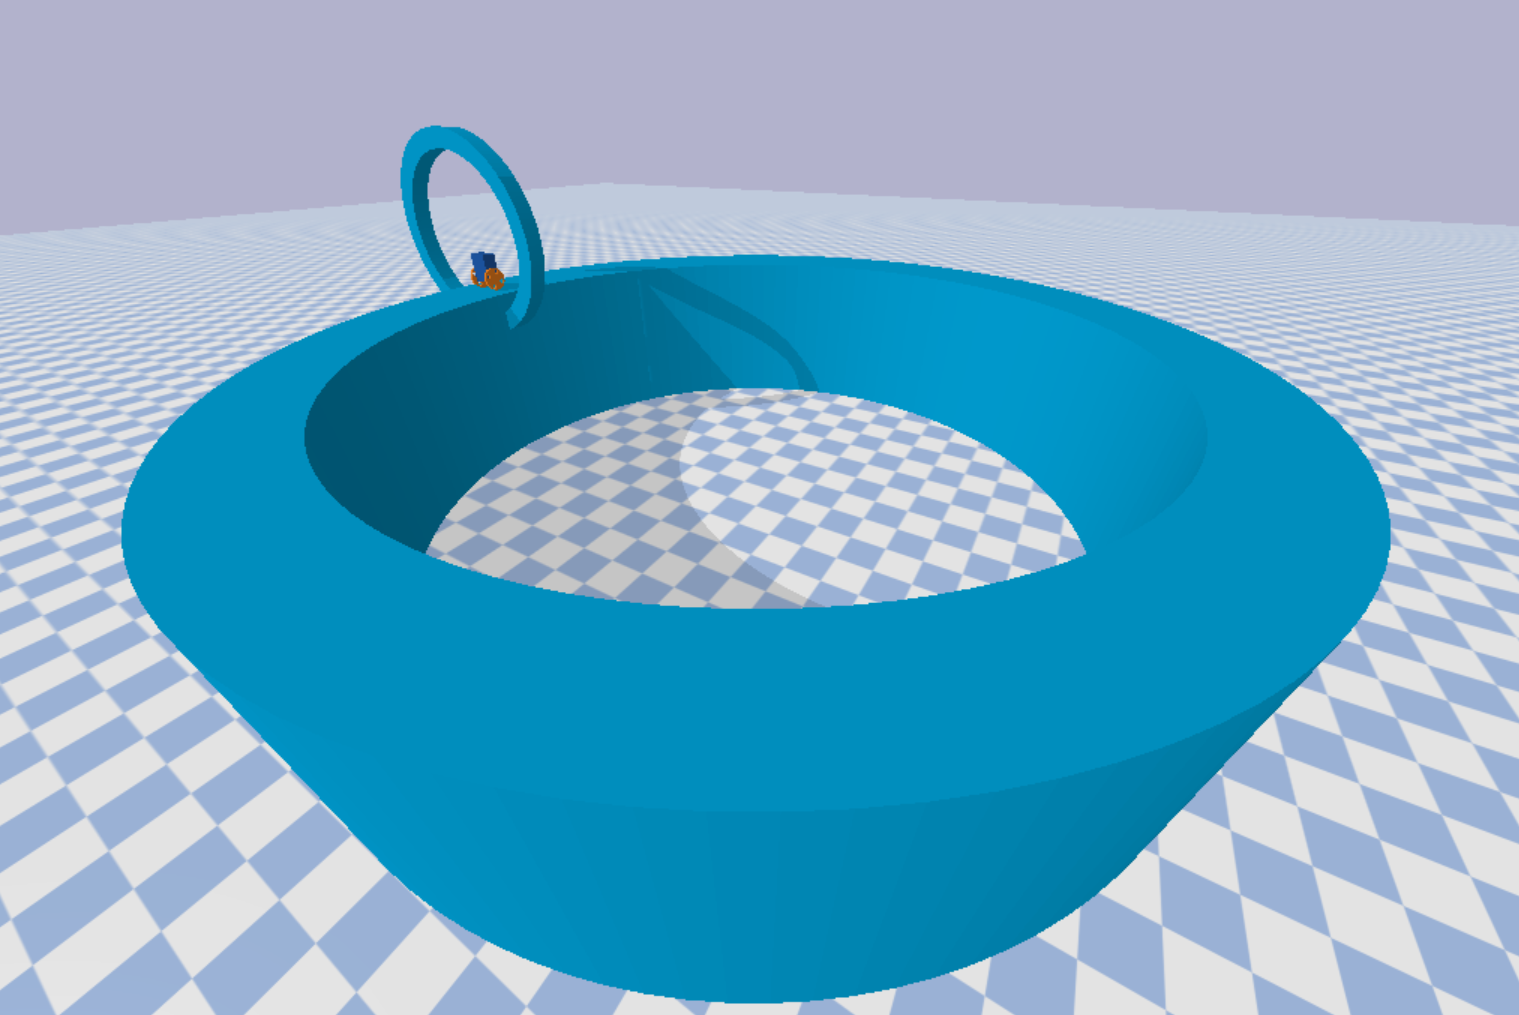
\includegraphics[scale=0.5]{ae353project2fig1}
    \caption{Snapshot of overall model, with robot on track}
    \label{fig:fig1}
\end{figure}
\\
If we assume incorrectly that the track is in fact straight rather than curved as shown above, the equations of motion are derived as:
\begin{center}
\begin{equation}
\begin{bmatrix} 
\dot{e}_\text{lateral} \\ 
\dot{e}_\text{heading} \\ 
\dot{v} \\ 
\dot{w} \\ 
\ddot{\theta} 
\end{bmatrix} = f(e_{lateral}, e_{heading}, v, w, \theta, \dot{\theta}, \tau_{l}, \tau_{r})
\end{equation}
\end{center}
where $f$ is\\
\begin{center}
\begin{equation}
f = 
\begin{bmatrix}v 
\sin{\left(e_{heading} \right)}\\
w\\
- \frac{2400 \tau_{l} + 2400 \tau_{R} + 2808 \left(\dot{\theta}^{2} + w^{2}\right) \sin{\left(\theta \right)} + 13 \left(250 \tau_{l} + 250 \tau_{r} - 195 w^{2} \sin{\left(2 \theta \right)} - 8829 \sin{\left(\theta \right)}\right) \cos{\left(\theta \right)}}{11700 \cos^{2}{\left(\theta \right)} - 12168}\\
\frac{32 \left(- 875 \tau_{l} + 875 \tau_{r} - 1443 \dot{\theta} w \sin{\left(2 \theta \right)} - 2925 v w \sin{\left(\theta \right)}\right)}{13 \left(3120 \sin^{2}{\left(\theta \right)} + 2051\right)}\\
\frac{42250 \tau_{l} + 42250 \tau_{r} - 32955 w^{2} \sin{\left(2 \theta \right)} + 300 \left(100 \tau_{l} + 100 \tau_{r} + 117 \left(\dot{\theta}^{2} + w^{2}\right) \sin{\left(\theta \right)}\right) \cos{\left(\theta \right)} - 1492101 \sin{\left(\theta \right)}}{1404 \left(25 \cos^{2}{\left(\theta \right)} - 26\right)}
\end{bmatrix}
\end{equation}
\end{center}
These equations of motion will be used for the design of the controller.

\section{\centering{Design}}
\begin{addmargin}[5em]{0em}
Design of the controller involves linearizing the equations of motion, showing said system is \end{addmargin} controllable, designing a stable controller, and implementing this controller to test in simulation. To linearize the equations of motion, we use the state space model as shown below:\\
\begin{center}
\begin{equation}
\dot{x} = Ax + Bu
\end{equation}
\end{center}
\begin{addmargin}[5em]{0em}
The state $x$ and input $u$ are used throughout. Because $x$ represents the state, we want to know \end{addmargin} the difference between the following and their equilibrium values: lateral error, heading error, forward speed, turning rate, pitch angle, and pitch rate. For the input $u$, we know differential drive robots are controlled by the torques in their wheels. The input will be the difference between the left and right torques and their equilibrium values. State matrix $x$ and input matrix $u$ are shown below:
\begin{center}
\begin{equation}
x = 
\begin{bmatrix} 
e_{lateral} - 
e_{lateral e} \\ 
e_{heading} -
e_{heading e} \\ 
v - v_{e} \\ 
w - w_{e} \\ 
\theta - \theta_{e}\\
\dot{\theta} - \dot{\theta_{e}}
\end{bmatrix}
\end{equation}
\begin{equation}
u = 
\begin{bmatrix} 
\tau_l - \tau_{le} \\
\tau_r - \tau_{re}  \\
\end{bmatrix}
\end{equation}
\end{center}
$\dot{x}$ is the derivative of the $x$ matrix. Because the equilibrium values are constants, they will disappear from the matrix. $\dot{x}$ is shown below:
\begin{center}
\begin{equation}
\dot{x} = 
\begin{bmatrix} 
\dot{e}_{lateral} \\ 
\dot{e}_{heading} \\ 
\dot{v}  \\ 
\dot{w}  \\ 
\dot{\theta} \\
\ddot{\theta}
\end{bmatrix} 
\end{equation}
\end{center}
Notice $\dot{x}$ is very similar to the equations of motion derived earlier. Using substitution, $\dot{x}$ effectively becomes:
\begin{center}
\begin{equation}
\begin{bmatrix}v 
\sin{\left(e_{heading} \right)}\\
w\\
- \frac{2400 \tau_{l} + 2400 \tau_{r} + 2808 \left(\dot{\theta}^{2} + w^{2}\right) \sin{\left(\theta \right)} + 13 \left(250 \tau_{l} + 250 \tau_{r} - 195 w^{2} \sin{\left(2 \theta \right)} - 8829 \sin{\left(\theta \right)}\right) \cos{\left(\theta \right)}}{11700 \cos^{2}{\left(\theta \right)} - 12168}\\
\frac{32 \left(- 875 \tau_{l} + 875 \tau_{r} - 1443 \dot{\theta} w \sin{\left(2 \theta \right)} - 2925 v w \sin{\left(\theta \right)}\right)}{13 \left(3120 \sin^{2}{\left(\theta \right)} + 2051\right)}\\
\dot{\theta}\\
\frac{42250 \tau_{l} + 42250 \tau_{r} - 32955 w^{2} \sin{\left(2 \theta \right)} + 300 \left(100 \tau_{l} + 100 \tau_{r} + 117 \left(\dot{\theta}^{2} + w^{2}\right) \sin{\left(\theta \right)}\right) \cos{\left(\theta \right)} - 1492101 \sin{\left(\theta \right)}}{1404 \left(25 \cos^{2}{\left(\theta \right)} - 26\right)}
\end{bmatrix}
\end{equation}
\end{center}
\begin{addmargin}[5em]{0em}
The $A$ and $B$ matrices were found by taking the jacobian of the $\dot{x}$ matrix with respect to the \end{addmargin} state matrix for $A$ and with respect to the input matrix for $B$. Next, the controllability matrix $W$ can now be found to determine if the system is controllable. The controllability matrix is defined as:
\begin{equation}
W = 
\begin{bmatrix}
B & AB & A^2B & ... & A^{n-1}B
\end{bmatrix}
\end{equation}
The system is considered controllable if the rank of this matrix $W$ is equal to the length of the matrix $A$.\\
\begin{addmargin}[5em]{0em}
Finally we need feedback to design the controller. A linear quadratic regulator (LQR) method \end{addmargin} was used to find the the optimal gain matrix. The equation for linear state feedback is:
\begin{equation}
u = -Kx
\end{equation}
The reason LQR was used is because it is extremely effective at finding optimal gain matrices while taking into account cost. The cost using LQR is shown as:
\begin{center}
\begin{equation}
\int_{0}^{\infty} (x(t)^TQx(t)+u(t)^TRu(t))^2 \,dt
\end{equation}
\end{center}
Once an optimal gain matrix was found, it was used to plug into equation 9, and the resulting $u$, which was the input, was used to control the robot. Due to the requirements and verification, certain equilibrium points were found through trial and error. 
\section{\centering{Results}}
\begin{addmargin}[5em]{0em}
Through trial and error, the appropriate equilibrium values were found to verify the requirements. \end{addmargin} In this case, all equilibrium values are zero, except for forward speed, which was found to be 1.7 m/s as the fastest the robot could go and still verify the requirements. These results are summarized in the $x_{equilibrium}$ matrix below:
\begin{equation}
x_{equilibrium} = 
\begin{bmatrix} 
e_{lateral e} = 0 \\ 
e_{heading e} = 0 \\ 
v_{e} = 1.7 \\ 
w_{e} = 0 \\ 
\theta_{e} = 0\\
\dot{\theta_{e}} = 0
\end{bmatrix}
\end{equation}
With these equilibrium values, the $A$ and $B$ matrices were found to be
\begin{equation}
A = 
\begin{bmatrix}
0.0 & 1.7 & 0.0 & 0.0 & 0.0 & 0.0\\0.0 & 0.0 & 0.0 & 1.0 & 0.0 & 0.0\\0.0 & 0.0 & 0.0 & 0.0 & -245.25 & 0.0\\0.0 & 0.0 & 0.0 & 0.0 & 0.0 & 0.0\\0.0 & 0.0 & 0.0 & 0.0 & 0.0 & 1.0\\0.0 & 0.0 & 0.0 & 0.0 & 1062.75 & 0.0
\end{bmatrix},
B = 
\begin{bmatrix}0.0 & 0.0\\0.0 & 0.0\\12.0726495726496 & 12.0726495726496\\-1.05014439485429 & 1.05014439485429\\0.0 & 0.0\\-51.460113960114 & -51.460113960114
\end{bmatrix}
\end{equation}
The controllability matrix $W$ was found to have a rank of 6, which is equal to the length of the $A$ matrix, confirming the system is controllable. Using LQR the optimal gain matrix $K$ was found to be
\begin{equation}
K = 
\begin{bmatrix}
-0.7071067 & -2.068364863 & -0.707106781 & -1.5714962 & -20.9867 & -1.1330208\\0.70710678 & 2.068364 & -0.7071067 & 1.57149 & -20.986741 & -1.133020
\end{bmatrix}
\end{equation}
\begin{addmargin}[5em]{0em}
The Verification is summarized by figure 2, which shows plots for lateral and heading errors,\end{addmargin} forward speed, turning rate, pitch angle, left and right wheel torques.
These plots clearly show the verification for this system and proves that the requirements are met. The maximum track error is 0.459 m, and the average speed is 1.5638 m/s. It should be noted, this is the result for initial conditions where the robot is turning left, the ground pitch is zero, initial speed is zero, initial lateral error is zero, initial heading error is zero, initial pitch is zero. 
\begin{figure}[h]
    \begin{center}
    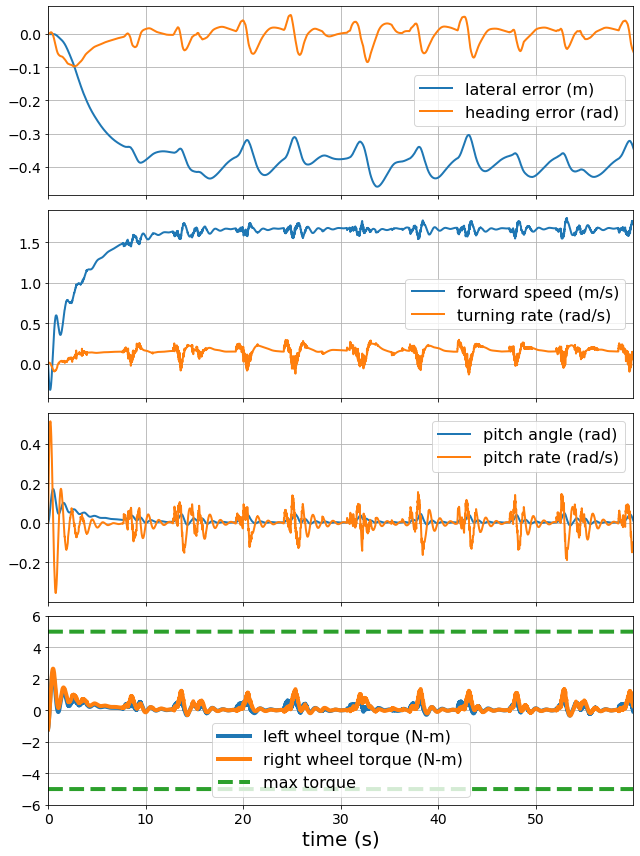
\includegraphics[scale=0.4]{ae353dp2plots}
    \caption{Plots for lateral and heading errors, forward speed, turning rate, pitch angle, left and right wheel torques for lateral error equilibrium value = 1.7}
    \label{fig:fig2}
    \end{center}
\end{figure}
\begin{addmargin}[5em]{0em}
How do the initial conditions affect the resulting motion? If the robot was turning right, and\end{addmargin} that is the only change in initial conditions, then we see nearly identical numbers, but opposite sign for things like lateral error, which of course is dependent on the direction it goes on the track. This was in the requirement, the need to satisfy the requirements in both directions. 
\begin{addmargin}[5em]{0em}
What about ground pitch? Changing the ground pitch very rapidly results in the robot falling \end{addmargin} off. A ground pitch as small as 0.1 radians results in the robot falling off \textit{if} the equilibrium values are kept the same. Through trial and error, going significantly slower by lowering the equilibrium forward rate value was the most effective way to counter this. However, this fails the requirement for maintaining a speed between 1 m/s and 3 m/s. 
\begin{addmargin}[5em]{0em}
Varying the initial speed of the robot had mixed results. Varying between 0 m/s and 2.5 m/s \end{addmargin} resulted in the robot being able to slow down fast enough to meet the requirements. Anything faster than that and the lateral error a few seconds after starting exceeds 0.5 m, even though after that it does recover and stay under 0.5 for the rest of the simulation. 
\begin{addmargin}[5em]{0em}
Initial lateral error ranging from -0.4 m to 0.4 m proved successful in verifying the requirements \end{addmargin} except for the condition that the robot would be turning left at a lateral error of 0.4. Interestingly, in this scenario, a lateral error of 0.4 results in the robot falling off. Dropping the lateral error to 0.3 solves this issue. 
\begin{addmargin}[5em]{0em}
Changing the initial heading error had no effects on the requirements except for the heading \end{addmargin} error requirement. The robot was able to successfully adjust quickly.
\\ 
\begin{addmargin}[5em]{0em}
Changing the initial pitch angle to anything greater than 0.5 radians or less than -0.3 radians \end{addmargin}resulted in the robot being unable to recover and falling flat. Between the range of -0.3 radians and 0.5 radians, the robot was able to recover quickly enough to satisfy the lateral error and speed requirements. That being said, this directly violates the pitch angle range in the requirements.

\section{\centering{Conclusion}}
\begin{addmargin}[5em]{0em}
The results show that the robot is able to verify all the requirements at the conditions met. \end{addmargin}Changing initial conditions very quickly makes some requirements impossible to verify, and some initial conditions themselves violate the requirements, such as making the initial pitch angle more than 0.2 radians. Room for improvement include the ability for the robot to handle larger ground pitches at faster speeds, going faster, the ability to gather more information about the track, and reduce lateral error throughout the simulation. The requirement was extremely strict and did not allow much room for movement. Realistically, there are some requirements that perhaps did not have to be so harsh, such as pitch angle or pitch rate. Real life application of something this stable could be a stable camera moving on two wheels. Indeed, this system does not seem superior to a four wheeled system, except its turning radius allows for extreme mobility in the lateral direction if needed. 
\section*{\centering{Acknowledgments}}
\begin{addmargin}[5em]{0em}
I would like to thank Professor Bretl for understanding of the controller and implementation of \end{addmargin} LQR. Base code for this project was given by Professor Bretl. Project tasks and deliverables were given on his website. The LQR method was taken directly from PraireLearn Homework 10. The process for finding the controllability matrix and rank to determine controllability was taken from PraireLearn Homework 8. The RobotController class was based off my RobotController class for Design Project 1. Special thanks to campuswire thread 249, unfortunately it is anonymous. Special thanks to campuswire thread 233 where Tyler Restoff describes an efficient way to create A and B matrices. Derivation of equations of motion taken directly from DeriveEOM.ipynb. 
\section*{\centering{References}}
\begin{enumerate}
  \item J. G. Batista et al., "Performance Comparison Between the PID and LQR Controllers Applied to a Robotic Manipulator Joint," IECON 2019 - 45th Annual Conference of the IEEE Industrial Electronics Society, Lisbon, Portugal, 2019, pp. 479-484, doi: 10.1109/IECON.2019.8927059.
\end{enumerate}

\end{document}

